\chapter{PHP language}
PHP is a general-purpose scripting language. It originated as a collection of Common Gateway Interface (CGI) scripts, written in PERL by Rasmus Lerdorf \citep{modern.php}. CGI scipt is a program executed by a server upon a request, whose output is then returned to a client \citep{cgi.perl}. It is essentially what makes server more than a collection of static resources \citep{cgi.perl}. Soon after their release, these PERL scripts were rewritten in C programming language to enhance their performance \citep{modern.php}. Since then, the underlying parser has been rewritten several times and many people were involved in implementing additional features and support libraries for this language \citep{php.manual}. 

PHP has been developed solely by individuals joining their effort. It has resulted in an organic growth of the language in a community of developers. On the one hand, environment in which the language grew caused many useful features and functions to be included in its core \citep{php.manual}. On the other hand, lack of supervision and pre-planning has produced significant inconsistency in function names and in order of functional parameters \citep{php.manual}. Furthermore, for over 20 years, no formal language specification defining correct language syntax existed \citep{Oscon2014}. This role was substituted by PHP's engine and the ``If it works, then it's fine" philosophy \citep{Oscon2014}. This task was addressed in 2014 and the resulting document is being further extended since by both, PHP community and the PHP Group \citep{Oscon2014, php.spec}. The PHP group is a comunity of developers that maintain both, PHP language repository on github and php.net web portal with all the necessary information about the language, from news about releases to actual language documentation.

Versioning of the language might prove to be quite confusing as the official name "PHP" language holds since version 3.0 \citep{php.manual}. Version 1.0 was more of a set of CGI tools than an actual standalone language and version 6.0 was left abandoned due to insufficient number of contributors considering the amount of work that promised unicode support brought \citep{php.manual, php.version6}. PHP versioning officially uses the [major].[minor].[release] scheme, but as the releases of the same major and minor version differ mostly in the number of bugs fixed, only the [major].[minor] scheme is generally used. Currently, PHP 7.4 is the latest stable released version, therefore, when speaking of PHP language without explicit version number mentioning, PHP version 7.4 is meant.

\paragraph{Execution}
PHP is an interpreted scripting programming language. Although both terms can be defined in several different ways, for the purpose of this text, we understand these terms as that the language was designed for a special-runtime environment without the need to be compiled. PHP scripts are executed by the Zend Engine, an open-source set of components than provide PHP language with tools for its processing and execution \citep{php.internals, modern.php}. It was written in C programming language by Zeev Suraski and Andi Gutmans for PHP version 4, after their previous collaboration with Rasmus Lerdorf on PHP version 3 \citep{php.manual}. Since then, 2 new versions of Zend Engine has been introduced, each time bringing new major version of PHP language \citep{php.manual, php.wiki}.

\paragraph{The Zend Engine}
Undoubtedly, the most important component of the Zend Engine is the Zend Virtual Machine (VM), responsible for interpretation of PHP script \citep{php.internals}. The first step the Zend VM performs when executing a PHP script is a lexical analysis \citep{advanced.php}. There it converts human-readable code to tokens for further procession. The parser then takes the stream of tokens and generates an intermediate code \citep{advanced.php}. Code optimizations can be performed during this stage, including resolving simple function calls with literal arguments, constant mathematical expressions folding or unreachable code removing \citep{advanced.php}. This part of PHP script processing is called the compilation phase, preceding the execution phase \citep{advanced.php}. After that, intermediate code in a form of an ordered array of opcodes is passed to the executor that steps through the array and executes each instruction in turn \citep{advanced.php}. 

One of the main features of the Zend Engine is its extensibility \citep{advanced.php}. The engine supports modifications either by using Zend extension API or through alterable function pointers \citep{advanced.php}. For example, both \texttt{zend{\_}compile} and \texttt{zend{\_}execute} functions that handle script processing phases are implemented internally as function pointers, making it possible for further custom overloading of these functions at runtime \citep{advanced.php}. 

The process of PHP application's execution is also illustrated in the following Figure.

\begin{figure}[h]
  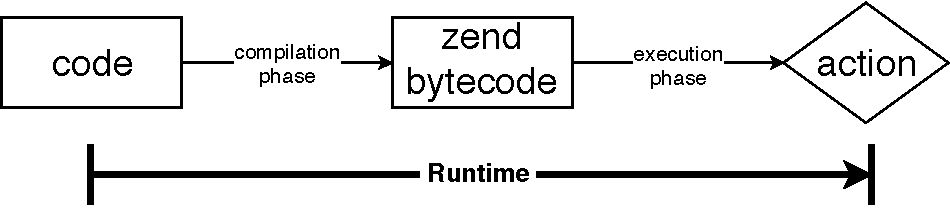
\includegraphics[width=\linewidth]{img/PHP.pdf}
  \caption{PHP's execution}
  \label{fig:php_execution}
\end{figure}





\section{Language features}
\paragraph{Object Oriented Programming}
Since the language version 5, Object Oriented Programming (OOP) is possible \citep{php.manual}. This enables developers to introduce another layer of abstraction above PHP code, possibly bringing higher level of organization and reducing maintenance burden. PHP supports all expected constructs of OOP such as Classes, Interfaces, Constructors and Inheritance \citep{php.manual}. On a class instantiation, \texttt{object} data type is created \citep{php.manual}. Every object is completely independent, holding its own properties and defined solely by a class it was instantiated from \citep{php.manual}. 

\paragraph{Type System}
PHP programming language is dynamically typed. This means that the language implicitly performs conversion between two types from different families, such as numbers and strings. This approach provides the language with additional flexibility and agility but does so at a cost of increased complexity and reduced safety. For instance, a developer with knowledge of how does inner conversion work is able to pass \texttt{integer 42} to a function expecting a \texttt{string} data type knowing, that the implicit conversion between the types will result in a \texttt{string 42}. On the other hand, an inexperienced developer might succeed comparing given variable with the equality operator \texttt{==} to \texttt{integer 42} without knowing that the variable actually holds \texttt{string 42}.

To decrease the required level of understanding of inner conversions and increase type safety, PHP provides several features for easier type manipulations and actively works on the development of the new ones. One of the most widely used amongst these features is the identity operator \texttt{===}, which extends the standard behaviour of equality operator with additional requirement for type equality of compared variables. Another much more recently added features are type hints, also called type declarations, and strict type checking \citep{php.manual}. These provide the means to specify both the expected types of function's parameters and its return type \citep{php.manual}. In case it is possible to perform an implicit conversion between the type provided and the type expected, the types declared in the function signature are by default for the purpose of backwards compatibility ignored \citep{php.manual}. However, strict type checking feature presents a way to force PHP interpreter to perform this additional type checking, enabling it to throw runtime errors on type mismatch, even when the implicit conversion is defined \citep{php.manual}.

Because of the dynamic nature of PHP data types, generic type relations are possible without any special constructs. However, this does only provide a way for a basic usage of generics in a form of what is in other languages called generic collections and generic function declarations. It does not allow for any further type relationships, such as bounding of generic types, to be declared and checked.

Special place between PHP data structures hold arrays. Internally, arrays are represented as ordered maps \citep{php.manual}. When provided, arrays use custom string or integer values as a keys for indexing, basic 0 based keys are used otherwise. Arrays with custom keys are called associative arrays. It is also notable that PHP does not throw an exception when float, boolean or null values are used as keys of an array \citep{php.manual}. Instead, as strings and integers are the only supported key types, implicit conversions between the types are performed \citep{php.manual}. On top of that, string keys representing a valid integer number are implicitly converted to integer keys \citep{php.manual}. 

\paragraph{Variables}
When a variable is declared by a standard syntactic mean of \$ sign followed by the case sensitive name of the variable, PHP disallows any explicit type definitions. Variable's type is determined by the context in which it is used, making it possible to seamlessly switch between types with a simple value assignment \citep{php.manual}. Moreover, PHP itself does not requite any formal declaration of variables \citep{php.manual}. The variable is automatically created the first time it is used in a scope and ceases to exist when it is set to null or \texttt{unset} method for this variable is called \citep{php.manual}. 

\paragraph{Request and Response}
As was mentioned before, PHP was designed to run on servers as a form of abstraction over the typical request-response based conversation between a client and a server. To abstract developers from actual HTTP request and to relieve them of the need for repetitive request parsing, several superglobal variables were built-in \citep{php.manual}. As the name suggests, these variables are always accessible, regardless the current scope. \texttt{\${\_}SERVER, \${\_}GET, \${\_}POST} and \texttt{\${\_}REQUEST} are all members of this group of variables. All of them contain parsed and ready to use data either about the request itself, such as uri or headers, or about data provided by the request, like submitted form fields and URL encoded parameters \citep{php.manual}.

Futhermore, PHP provides means to easily create HTTP response in just a few lines, taking care of the actual HTTP response creation itself. For instance the \texttt{header} function accepts a string as a parameter and setts it as one of returned response's headers \citep{php.manual}. Additionally, the most profound PHP construct \texttt{echo} is also used in this context as it takes its parameters and appends them to the response's body \citep{php.manual}. 



\section{Composer}
Composer is a tool for managing dependencies in PHP. Composer works with libraries, sometimes referred to as packages or projects, on a per-project basis. This is what differs the tool from traditional Linux package managers such as APT as they usually install packages globally, for computer's operating system, making it more similar to NPM or YARN managers \citep{composer.docs}. These libraries composer works with are zip archives of \texttt{composer.json} configuration file, code, optional \texttt{composer.lock} file and any other code-related resources \citep{composer.docs}.

When composer executes a command, in most cases either input or output of the command is a \texttt{composer.json} configuration file or its update. This file provides means to specify basic information about the package like its name, description, dependencies or type, which can be of project, library, metapackage or composer-plugin \citep{composer.docs}. It can be also used to specify additional package repositories and to define scripts as aliases of command-line executables whose execution can be linked to composer's commands \citep{composer.docs}. Where some commands, like \texttt{install} or \texttt{update}, do require the \texttt{composer.json} file's existence prior to their execution, as their functionality lays in loading current package's configuration and acting upon it, other commands, such as \texttt{require} or \texttt{create-project}, only settle for their arguments and the \texttt{composer.json} file's creation or modification is a result of their work \citep{composer.docs}.

Third-party libraries installation is done via require command suffixed with library's name and an optional version number \citep{composer.docs}. When resolving a package, one possible outcome is composer finding a zip archive of this library, in which case its contents is unzipped to a \texttt{vendor/[libraryName]} folder \citep{composer.docs}. Sometimes a metapackage is found instead. These are empty packages containing just a composer.json file with basic information and a list of dependencies and a \texttt{readme.md}, as they are usually hosted on version control services \citep{composer.docs}. In this case, new instance of composer is created for this \texttt{composer.json} configuration file and installation of listed dependencies is triggered. Both ways result in one or more added libraries to vendor directory. Every package installation or update also result in either update or creation of a \texttt{composer.lock} file. Where \texttt{composer.json} file holds a list of packages and basic information about current project, the \texttt{composer.lock} file notes actual version of each package resolved by the composer and can be therefore used to ensure that the same set of dependencies is installed in all the instances of the project. 





\section{Symfony framework}
Symfony is a PHP framework for web application development. It is built on top of the Symfony Components, a set of reusable PHP libraries \citep{symfony.reference}. Each library provides certain functionalities and many of them are completely independent, making it possible to use them without the need for using the Symfony framework itself \citep{symfony.reference}. This universality gave birth to many new web frameworks such as Laravel or Drupal version 8, which are built atop the Symfony Components as well \citep{symfony.reference}.

The Symfony framework evolves a lot each time a major version is released but its philosophy remains. It is to give developers full control over the project's configuration, from the directory structure to a set of used libraries \citep{symfony.reference}. When the work on the project began, Symfony 4.2 was the latest stable version of the framework released, for this reason, further description would primarily focus on this version.


\paragraph{Installation}
Bare bones Symfony application is created via composer, more precisely the \texttt{create-project} command with either the \texttt{symfony/website-skeleton} or the \texttt{Symfony/skeleton} argument \citep{symfony.reference}. When executed, composer downloads predefined set of core libraries that handle base framework functionality \citep{symfony.reference}. After that, everything from routing set-up to additional libraries downloading with the \texttt{composer require} command is up to developer.


\paragraph{Request and Response}
Symfony's way of request-response conversation handling is nothing more than an object-oriented abstraction of the PHP's one \citep{symfony.reference}. For this purpose, the \texttt{Request} and the \texttt{Response} classes, with specialized functions for request and response manipulation were introduced \citep{symfony.reference}. These two classes are part of a Symfony Component called \texttt{symfony/http-foundation}, which is included by composer on application's skeleton installation \citep{symfony.reference}.

\paragraph{Front Controller}
Traditional small PHP applications usually follow a simple pattern, where each site's page is represented by a physical file, for example \texttt{index.php}. As the size of an application increases, this approach brings an overhead in the form of code repetition, complicated route changing and overall decreased flexibility. For this purpose, larger application may define single PHP script called Front Controller, that handles every incoming request and calls another, more specialized controllers that provide actual response \citep{advanced.php}. 

The Symfony framework is no exception to this approach. However, instead of specialized controller calling, everything Symfony's front controller does is booting Symfony and passing information about the request \citep{symfony.reference}. This is done by executing the \texttt{src\textbackslash{}Kernel.php} script \citep{symfony.reference}. Afterwards, \texttt{Kernel.php} uses the Routing component to interpret the request and to resolve the appropriate controller to be called \citep{symfony.reference}. Finally, based on request's method and parameters, selected function from the controller is executed, resulting in the Response object, that is converted by the Symfony framework to the HTTP response and sent back to the client \citep{symfony.reference}.




\section{Twig}
TWIG is a PHP library used to combine template files with data model to produce HTML documents. In other words, it is a template engine. Its syntax consists of HTML extended with TWIG code and three special delimiters. 

\paragraph{Output delimiter}
The first one is \texttt{\string{\string{...\string}\string}}, which is used for outputting results of expressions \citep{twig.docs}. These can be either variable names or function calls \citep{twig.docs}. TWIG has a small set of predefined functions \citep{twig.docs}. Some have straightforward functionality and self-explaining name such as dump and max, where other are much more complex, like include, resulting in included TWIG template loading, generating and embedding the result in the current template \citep{twig.docs}. Every expression can be suffixed with arbitrary number of \texttt{|[filterName]} expressions to further process result before its outputting \citep{twig.docs}. TWIG comes with approximately 40 filters such as upper, split and replace \citep{twig.docs}. The predefined filters and functions usually cover the basic usage of the engine. However, extending built-in functions and filters is also possible by writing PHP script extending the \texttt{AbstractExtension} class and defining the \texttt{getFilters} or the \texttt{getFunctions} method, which is used to link the filter's or the function's implementation method to its alias through which it can be further used \citep{twig.docs}. 

\paragraph{Other delimiters}
The second delimiter is \texttt{\string{\%...\%\string}}, used for executing statements and controlling the flow of a program \citep{twig.docs}. Supported structures are for instance \texttt{\string{\% for - in - \%\string}...\string{\% endfor \%\string}}, \texttt{\string{\% if - \%\string}...\string{\% endif \%\string}} or \texttt{\string{\% set - = - \%\string}} \citep{twig.docs}. Finally, comments are supported via the \texttt{\string{\# ... \#\string}} syntax \citep{twig.docs}.


\paragraph{Template inheritance}
The most useful and powerful feature of TWIG is template inheritance. This allows to build a template acting as a basis that child templates further extend. Such template may contain all the common elements of a site - header, footer and a navigation bar. Furthermore, it can define blocks with \texttt{\string{\% block - \%\string}...\string{\% endblock \%\string}} syntax, whose content can be either fully overwritten by child templates or combined with child's one via \texttt{\string{\string{ parent() \string}\string}} function \citep{twig.docs}. Inheritance is enabled for selected templates by specifying a parent template with \texttt{\string{\% extends - \%\string}} construct in the beginning of each child template \citep{twig.docs}.

\paragraph{Environment}
Environment is a object used for storing the configuration with possible extensions, loading and rendering of a template \citep{twig.docs}. The lookup and loading of a template is performed by a loader, class implementing the \texttt{\textbackslash{}Twig\textbackslash{}Loader\textbackslash{}LoaderInterface} interface, which is provided as a first parameter to the \texttt{\textbackslash{}Twig\textbackslash{}Environment} class constructor \citep{twig.docs}. Template is loaded with the \texttt{load} method of the Environment class and rendered with the \texttt{render} method of the \texttt{\textbackslash{}Twig\textbackslash{}TemplateWrapper} class, whose instance is returned by the load method \citep{twig.docs}. The \texttt{render} method takes either one parameter - an associative array of variable names and values that are to be provided to rendered template, in which case it acts as described before, or two parameters - template name and an array \citep{twig.docs}. The second form wraps both the loading and the rendering of the template internally, returning directly a rendered string of HTML markup \citep{twig.docs}. The \texttt{templateWrapper} class also provides a self-explanatory method \texttt{renderBlock} \citep{twig.docs}.

\paragraph{} A simple example of Twig template providing a header for calendar table is provided in the following Listing.

\begin{center}
\lstset{language=XML,
	morekeywords={colspan, class, title}}
\begin{lstlisting}[caption={Twig example},captionpos=b]
<thead>
	<tr>
		<th colspan="7" class="month">
			{{ monthnames[month].full }}
        </th>
    </tr>
    <tr>
        {% for dow in range(0, 6) %}
        	{% set day = (dow + firstDay) % 7 %}
            <th class="
            	day {% if (day == 6 or day == 0) %}weekend{% endif %}
            ">
            	<span title="{{ daynames[day].full }}">
            		{{ daynames[day].short }}
            	</span>
            </th>
       {% endfor %}
	</tr>
</thead>
\end{lstlisting}
\end{center}

